\documentclass[11pt, xcolor={dvipsnames}]{beamer}

\mode<presentation> {
\usetheme{CambridgeUS}
\usecolortheme{whale}
}

\setbeamercolor*{structure}{bg=NavyBlue!20,fg=NavyBlue}

\setbeamercolor*{palette primary}{use=structure,fg=white,bg=structure.fg}
\setbeamercolor*{palette secondary}{use=structure,fg=white,bg=structure.fg!75}
\setbeamercolor*{palette tertiary}{use=structure,fg=white,bg=structure.fg!50!black}
\setbeamercolor*{palette quaternary}{fg=white,bg=black}

\setbeamercolor{section in toc}{fg=black,bg=white}
\setbeamercolor{alerted text}{use=structure,fg=structure.fg!50!black!80!black}

\setbeamercolor{titlelike}{parent=palette primary,fg=structure.fg!50!black}
\setbeamercolor{frametitle}{bg=gray!10!white,fg=Blue}

\setbeamercolor*{titlelike}{parent=palette primary}

%\usepackage[utf8]{inputenc}

\usepackage{graphicx} 
\usepackage{wrapfig}
\usepackage{booktabs} 
\usepackage{cite}
\usepackage{mathtools}
\usepackage{setspace}
\usepackage{chemformula}
\usepackage[utf8]{inputenc}
\usepackage{siunitx} %pretty measurement unit rendering
\usepackage{ragged2e}
\usepackage[font=scriptsize,justification=justified]{caption}
\usepackage{array,booktabs,tabularx}
\usepackage{algorithmic}
\usepackage[linesnumbered,ruled]{algorithm2e}
\usepackage{changepage}
\usepackage{multicol}
\SetKwRepeat{Do}{do}{while}%
\SetAlgoNoEnd%

\makeatletter
\newcommand{\setalgomidrulecolor}[1]{\colorlet{midrulecolor}{#1}}
\renewcommand{\algocf@caption@ruled}{%
  \box\algocf@capbox{\color{midrulecolor}\kern\interspacetitleruled\hrule
    width\algocf@ruledwidth height\algotitleheightrule depth0pt\kern\interspacealgoruled}}
\makeatother
\setalgomidrulecolor{white!30}

\newcommand{\setF}{{\mathcal F}}
\newcommand{\setG}{{\mathcal G}}
\newcommand{\setH}{{\mathcal H}}
\newcommand{\setL}{{\mathcal L}}
\newcommand{\setR}{{\mathcal R}}
\newcommand{\setT}{{\mathcal T}}
\newcommand{\setX}{{\mathcal X}}
\newcommand{\setY}{{\mathcal Y}}
\newcommand{\setZ}{{\mathcal Z}}
\newcommand{\bx}{{\mathbf x}}
\newcommand{\by}{{\mathbf y}}
\newcommand{\bz}{{\mathbf z}}
\newcommand{\I}{{\mathbb I}}
\newcommand{\realnum}{{\mathbf R}}
\newcommand{\posnum}{{\mathbb N^+}}
\newcommand{\argmin}{{\arg\min}}
\DeclarePairedDelimiter{\norm}{\lVert}{\rVert}
\newcommand{\Ha}{\mathcal{H}_1^B}
\newcommand{\empproc}{{\mathbb P}} % empirical process
\newcommand{\rproc}{{\mathbb R}} % empirical process
\DeclareMathOperator{\conv}{co}
\DeclareMathOperator{\lin}{lin}
\DeclareMathOperator{\bin}{bin}
\DeclareMathOperator{\hardtanh}{hardtanh}
\usepackage{color}
\newcommand{\comment}[1]{{\color{red} #1}}
\newcommand{\grad}{\nabla}
\newcommand{\funcgrad}{D}

\newcolumntype{Z}{>{\centering\arraybackslash}X} % centered tabularx columns
\sisetup{per=frac,fraction=sfrac}



\institute[] 
{
%\vspace*{-0.35cm}
%\includegraphics[width=1.8cm]{img/Qut_Logo}
%\vspace*{0.55cm}\\

Tan Nguyen (Queensland University of Technology) 
\vspace*{0.3cm}\\ Nan Ye (University of Queensland) 
\vspace*{0.3cm}\\ Peter Bartlett (UC Berkeley)
}
\date{\today}


%\AtBeginSection[]
%{
%\begin{frame}
%\frametitle{Greedy Convex Ensemble}
%\tableofcontents[currentsection, hideallsubsections]
%\end{frame}
%}

% ==========================================================
\title[IJCAI-PRICAI 2020]{Greedy Convex Ensemble} 

\author[T Nguyen, N Ye, P Bartlett]{
%Queensland University of Technology
} 



\begin{document}

\begin{frame}
\titlepage 
\end{frame}

%\begin{frame}{Content} 
%\tableofcontents[hideallsubsections]
%\end{frame}

% ==========================================================
\section{Greedy Convex Ensemble} 

% ============================
\begin{frame}{The Problem}
"Learning a convex ensemble of basis models"

\noindent
\begin{minipage}[t]{0.35\textwidth}
\includegraphics[clip, trim=1cm 8cm 23cm 0cm, width=0.9\textwidth]{fig1}
\end{minipage}%
\begin{minipage}[t]{0.6\textwidth}
\vspace{-3.8cm}
Given some set $\setG$ of basis models.
\vspace{0.1cm}\\
\textit{\underline{Linear hull}}, $\lin(\setG),$ is the set of all possible linear combinations of models in $\setG$
\begin{itemize}
\item $\lin(\setG)$ of even simple basis models is an universal approximator
\end{itemize}

\textit{\underline{Convex hull}}, $\conv(\setG),$ is the set of all possible convex combinations of models in $\setG$
\begin{itemize}
\item Convex hull is a subset of the linear hull
\item Theoretical: Capacity? Generalization? 
\item Empirical: How to learn from a convex hull? Any advantages?
\end{itemize}
\end{minipage}

\end{frame}

% ============================
\begin{frame}{Capacity of Convex Hulls}

\emph{Proposition 2:} For linear threshold basis models, \\
\hspace{2.5cm}i.e. $ \setG = \{\I(\theta^{\top} x \ge t): \theta \in \realnum^{d}, t \in \realnum\},$
\begin{itemize} 
\item Linear hulls: infinite pseudodimension and Rademacher complexity
\item Convex hulls: infinite pseudodimension, finite Rademacher complexity 
\end{itemize}
\vspace{0.5cm}

\emph{Implication:} 
\begin{itemize} 
\item Linear hulls: unbounded capacity, thus prone to overfitting.
\item Convex hulls: rich but bounded capacity, can be seen as a regularized version of linear hulls.
\end{itemize}

\end{frame}

% ============================
\begin{frame}{Generalization Bound}

\emph{\underline{Theorem 2:}} 	With probability at least $1 - \delta$, for all $f \in \conv(\setG),$ \\
\hspace{2.5cm}$R(f) - R(f^{*}) \le R_{n} (f) - R_{n}(f^{*}) + \frac{c}{\sqrt{n}},$ \\
where 
$c = {2 c_{\phi} B \left(\sqrt{2 \ln(1/\delta)} + D\sqrt{p} + 2\right)}$ 
and $f^*$ is Bayes optimal.
\vspace{0.2cm}\\
$\Longrightarrow$ \emph{Minimizing empirical risk $R_n(f)$ over the convex hull $\conv(\setG)$ results in minimizing the bound of the expected risk $R(f)$.}
\vspace{0.5cm}\\

\emph{\underline{Theorem 3:}} Let $\hat{f} = \argmin_{f \in \conv(\setG)} R_{n}(f)$, and $h^{*} = \argmin_{f \in \conv(\setG)} R(f)$, 
then with probability at least $1 - \delta,$
\hspace{0.2cm} $R(\hat{f}) \le R(h^{*}) + \frac{c}{\sqrt{n}}.$
\vspace{0.2cm}\\
$\Longrightarrow$ \emph{In $\conv(\setG)$, the empirical risk minimizer $\hat f$ converges to the expected risk minimizer $h^*$ at the rate $O(1/\sqrt n)$.}

\end{frame}


% ============================
\begin{frame}{Algorithms to Learn GCE}
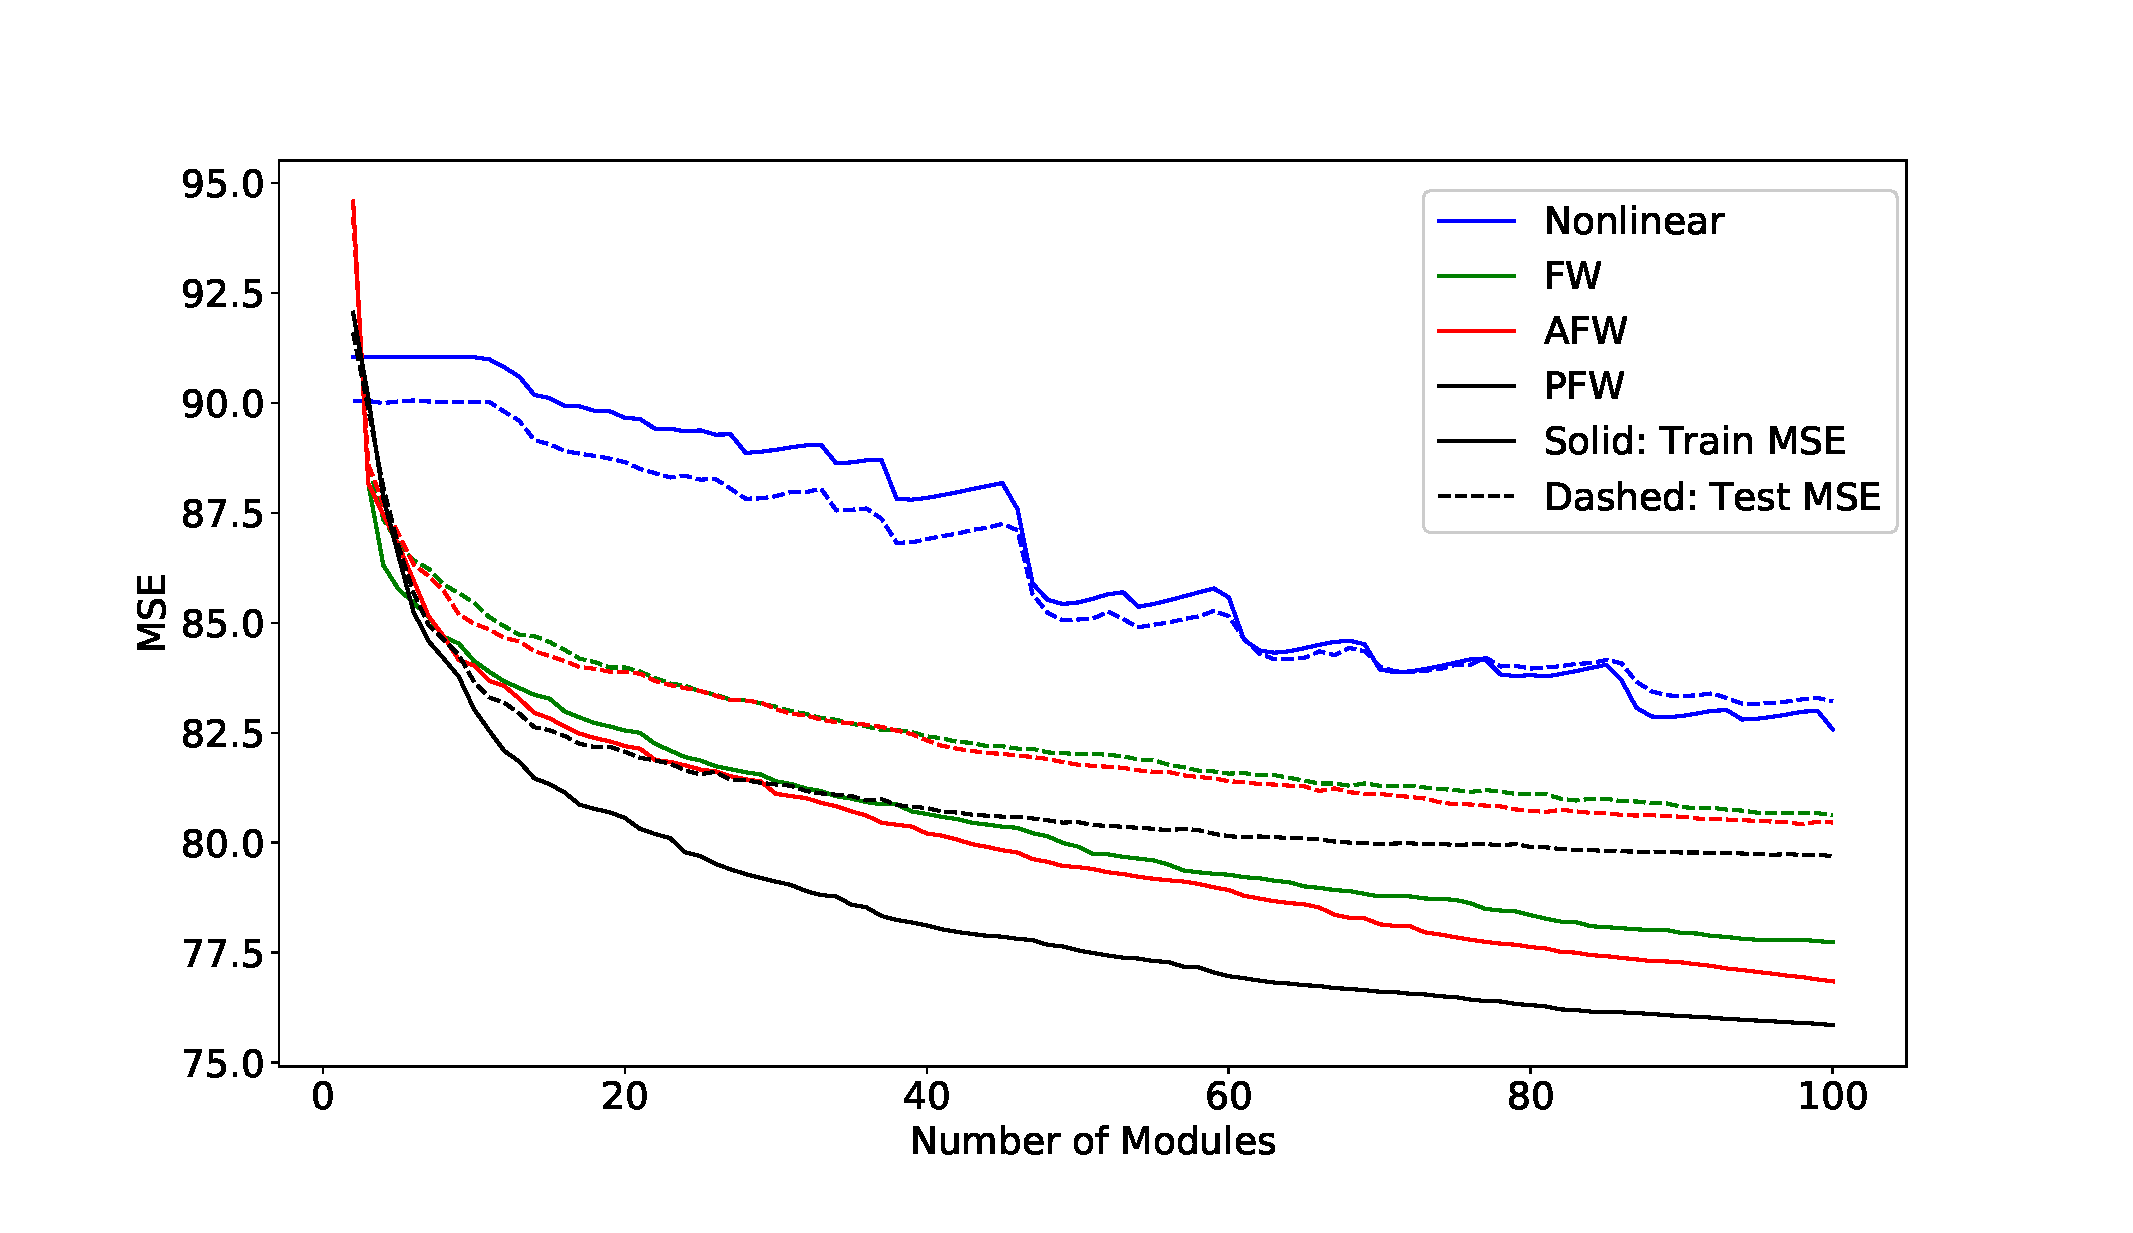
\includegraphics[width=\columnwidth]{nips_greedy_algs_msd.eps}
\end{frame}

% ============================
\begin{frame}{Performance Comparison}
\footnotesize{
\begin{table}[H]
\centering
\begin{tabular}[t]{lrrrrrrrr} 
\toprule
\textbf{Datasets} & \#\textbf{Samples} & \textbf{GCE} & \textbf{XGBoost} & \textbf{RForest} & \textbf{NN} & \textbf{ConvNet} \\
\midrule
diabetes & 442 & \textbf{42.706} & 46.569 & 49.519 & 43.283 & 44.703 \\
boston & 506 & \textbf{2.165} & 2.271 & 2.705 & 2.217 & 2.232 \\
ca\_housing &20,640& 0.435 & \textbf{0.393} & 0.416 & 0.440 & 0.437  \\
msd & 515,345& \textbf{6.084} & 6.291 & 6.462 & 6.186 & 7.610 \\
\midrule
iris & 150 & \textbf{0.00} & 6.67 & 6.67 & 3.33 & 10.00  \\
wine & 178 & \textbf{0.00} & 2.78 & 2.78 & \textbf{0.0} & \textbf{0.0}  \\
breast\_cancer & 569 & \textbf{3.51} & 4.39 & 8.77 & 3.51 & 4.39 \\
digits & 1,797 & 2.78 & 3.06 & \textbf{2.50} & 3.33 & 3.06 \\
cifar10\_f & 60,000 & \textbf{4.86} & 5.40 & 5.16 & 5.00 & 4.92 \\
mnist & 70,000 & 1.22 & 1.66 & 2.32 & 1.24 & \textbf{1.11} \\
covertype & 581,012 & 26.70 & 26.39 & 27.73 & 26.89 & \textbf{26.56} \\
kddcup99 & 4,898,431 & \textbf{0.01} & \textbf{0.01} & \textbf{0.01} & \textbf{0.01} & \textbf{0.01}\\
\bottomrule
\end{tabular}
\end{table}
}
\end{frame}


% ==========================================================
%\nocite{*}
%\begin{frame}[allowframebreaks]{Reference}
%\bibliographystyle{apalike}
%\bibliographystyle{agsm} 
%\bibliography{bib.bib}
%\begin{thebibliography}{BH}
 
%\bibitem{Audi10} Audibert J. and Bubeck S.:\textit{ Best Arm Identification in Multi-Armed Bandits}, COLT - 23th Conference on Learning Theory, 2010
%\end{thebibliography}
%\printbibliography
%\end{frame}


% ==========================================================
\begin{frame}
\titlepage 
\end{frame}

\end{document}